\appendix
\chapter{Kansai Joint Seminar Poster}
\label{appendix1}

\begin{figure}[H]
\begin{center}
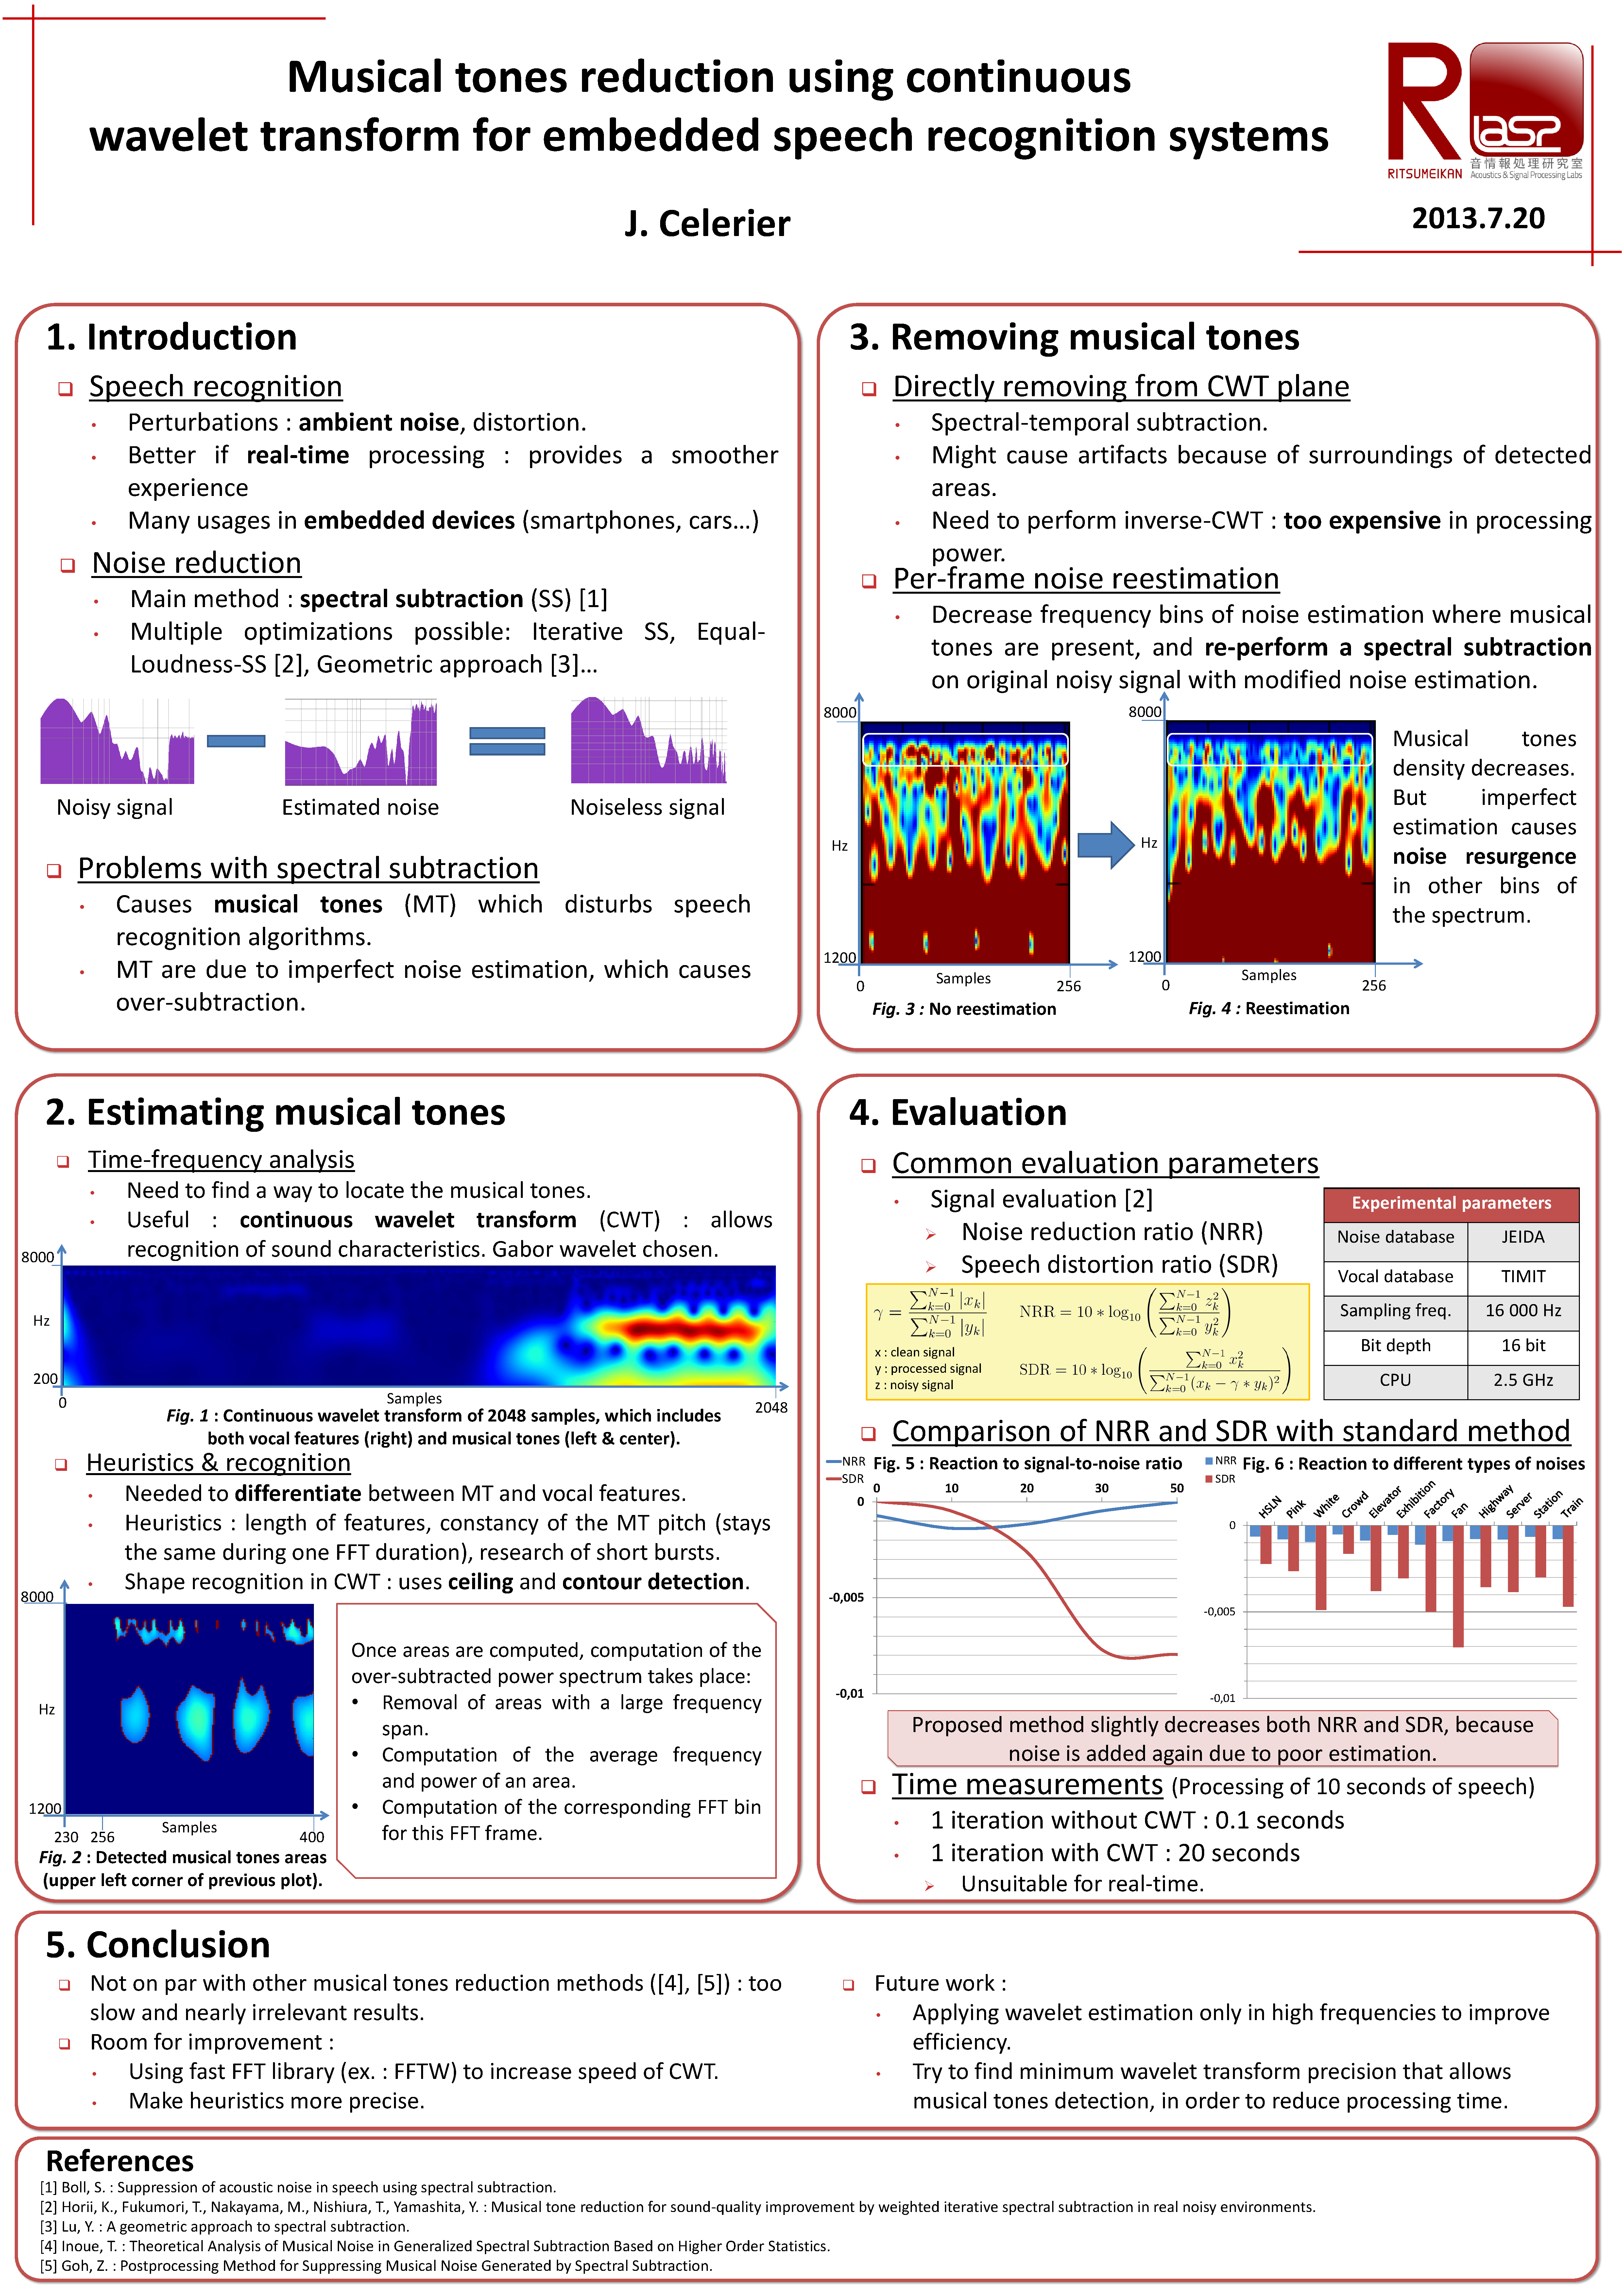
\includegraphics[scale=0.2]{images/poster.pdf}
\caption{The poster I made}
\label{diag_api_chords}
\end{center}
\end{figure}
\newpage
\chapter{Warnings used for compilation of the library}
\label{appendix2}
\begin{lstlisting}[language=python]
-Wall
-pedantic
-Wextra
-Weffc++
-Wall
-Wcast-align
-Wcast-qual
-Wchar-subscripts
-Wcomment
-Wconversion
-Wdisabled-optimization
-Wformat
-Wformat=1
-Wformat-nonliteral
-Wformat-security
-Wformat-y2k
-Wimport
-Winit-self
-Winline
-Winvalid-pch
-Wunsafe-loop-optimizations
-Wmissing-braces
-Wmissing-field-initializers
-Wmissing-format-attribute
-Wmissing-include-dirs
-Wmissing-noreturn
-Wpacked
-Wparentheses
-Wpointer-arith
-Wredundant-decls
-Wreturn-type
-Wsequence-point
-Wshadow
-Wsign-compare
-Wstack-protector
-Wstrict-aliasing=3
-Wswitch
-Wswitch-default
-Wswitch-enum
-Wtrigraphs
-Wuninitialized
-Wunknown-pragmas
-Wunreachable-code
-Wunused
-Wunused-function
-Wunused-label
-Wunused-parameter
-Wunused-value
-Wunused-variable
-Wvariadic-macros
-Wvolatile-register-var
-Wwrite-strings
\end{lstlisting}

\bibliographystyle{plain}
\bibliography{biblio}